\documentclass[12pt,a4paper]{article}
\usepackage[utf8]{inputenc}
\usepackage[T1]{fontenc}
\usepackage{geometry}
\usepackage{graphicx}
\usepackage{xcolor}
\usepackage{titlesec}
\usepackage{fancyhdr}
\usepackage{hyperref}
\usepackage{listings}
\usepackage{tcolorbox}
\usepackage{enumitem}
\usepackage{tabularx}
\usepackage{booktabs}
\usepackage{amsmath}
\usepackage{amssymb}
\usepackage{float}
\usepackage{tikz}
\usepackage{pgfplots}
\usepackage{url}

% Page geometry
\geometry{margin=1in}

% Colors
\definecolor{primaryblue}{RGB}{0,123,255}
\definecolor{secondarygreen}{RGB}{40,167,69}
\definecolor{warningyellow}{RGB}{255,193,7}
\definecolor{dangerred}{RGB}{220,53,69}
\definecolor{lightgray}{RGB}{248,249,250}
\definecolor{darkgray}{RGB}{52,58,64}

% Hyperref setup
\hypersetup{
    colorlinks=true,
    linkcolor=primaryblue,
    filecolor=magenta,
    urlcolor=primaryblue,
    citecolor=primaryblue,
    pdftitle={PurrfectMatch Technical Documentation},
    pdfauthor={Development Team},
    pdfsubject={Pet Adoption Platform},
    pdfkeywords={.NET, React, TypeScript, Clean Architecture, Pet Adoption, SignalR, Stripe}
}

% Custom title formatting
\titleformat{\section}
{\Large\bfseries\color{primaryblue}}
{\thesection}{1em}{}

\titleformat{\subsection}
{\large\bfseries\color{secondarygreen}}
{\thesubsection}{1em}{}

% Code listing style
\lstdefinestyle{codestyle}{
    backgroundcolor=\color{lightgray},
    commentstyle=\color{darkgray},
    keywordstyle=\color{primaryblue},
    numberstyle=\tiny\color{darkgray},
    stringstyle=\color{secondarygreen},
    basicstyle=\ttfamily\footnotesize,
    breakatwhitespace=false,
    breaklines=true,
    captionpos=b,
    keepspaces=true,
    numbers=left,
    numbersep=5pt,
    showspaces=false,
    showstringspaces=false,
    showtabs=false,
    tabsize=2,
    frame=single,
    rulecolor=\color{lightgray}
}

\lstset{style=codestyle}

% Header and footer
\pagestyle{fancy}
\fancyhf{}
\rhead{\textcolor{primaryblue}{PurrfectMatch Technical Documentation}}
\lhead{\textcolor{secondarygreen}{\leftmark}}
\cfoot{\thepage}

\begin{document}

% Title page
\begin{titlepage}
    \centering
    \vspace*{2cm}
    
    {\Huge\bfseries\color{primaryblue} PurrfectMatch}\\[0.5cm]
    {\Large\color{secondarygreen} Pet Adoption Platform}\\[2cm]
    
    {\huge\bfseries Technical Documentation}\\[1cm]
    
    \begin{tcolorbox}[colback=lightgray, colframe=primaryblue, width=0.8\textwidth]
        \centering
        \textbf{A comprehensive full-stack pet adoption platform built with modern technologies}\\[0.5cm]
        
        \begin{tabular}{@{}ll@{}}
            \textbf{Backend:} & .NET 8.0, ASP.NET Core, Entity Framework Core \\
            \textbf{Frontend:} & React 19.0, TypeScript 5.7, Material-UI \\
            \textbf{Database:} & Microsoft SQL Server \\
            \textbf{Cloud:} & Azure Blob Storage \\
            \textbf{Payments:} & Stripe Integration \\
            \textbf{Real-time:} & SignalR \\
            \textbf{Architecture:} & Clean Architecture, DDD Principles
        \end{tabular}
    \end{tcolorbox}
    
    \vfill
    
    {\Large Development Team}\\[0.5cm]
    {\large \today}
\end{titlepage}

\newpage
\tableofcontents
\newpage

\section{Executive Summary}

PurrfectMatch is a modern, full-stack pet adoption platform designed to connect pet lovers with their ideal companions from shelters and rescues worldwide. The platform is built using industry-standard technologies and follows Clean Architecture principles to ensure maintainability, scalability, and testability.

\subsection{Project Overview}

The system facilitates pet adoption through comprehensive features including:
\begin{itemize}
    \item Advanced pet search and filtering capabilities
    \item Shelter management and verification systems
    \item Adoption application processing
    \item Real-time notifications via SignalR
    \item Integrated donation system with Stripe
    \item Community features including posts and reviews
    \item Administrative analytics and reporting
\end{itemize}

\section{System Architecture}

\subsection{Architectural Pattern}

PurrfectMatch implements \textbf{Clean Architecture} with Domain-Driven Design (DDD) principles, ensuring clear separation of concerns and maintainable code structure.

\begin{figure}[H]
    \centering
    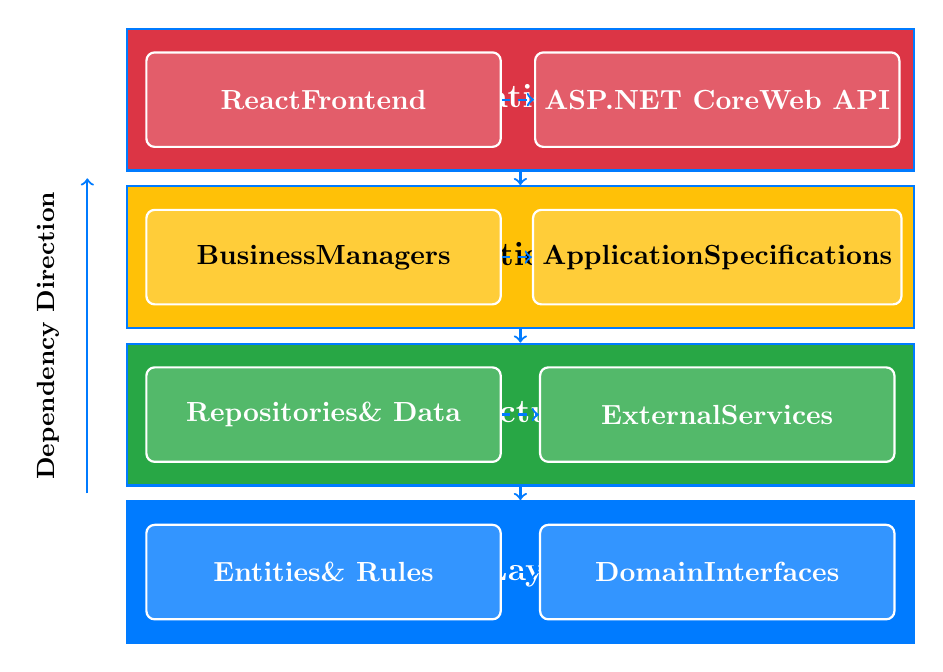
\begin{tikzpicture}[
        layer/.style={rectangle, draw=primaryblue, thick, minimum width=10cm, minimum height=1.8cm, 
                     text centered, font=\large\bfseries, text=white},
        sublayer/.style={rectangle, draw=white, thick, minimum width=4.5cm, minimum height=1.2cm, 
                        text centered, font=\normalsize\bfseries, text=white, rounded corners=3pt},
        arrow/.style={->, thick, color=primaryblue}
    ]
        % Draw main architecture layers with different colors
        \node[layer, fill=dangerred] (presentation) at (0,6) {Presentation Layer};
        \node[layer, fill=warningyellow, text=black] (application) at (0,4) {Application Layer};
        \node[layer, fill=secondarygreen] (infrastructure) at (0,2) {Infrastructure Layer};
        \node[layer, fill=primaryblue] (domain) at (0,0) {Domain Layer (Core)};
        
        % Add sublayers for presentation
        \node[sublayer, fill=dangerred!80] (web) at (-2.5,6) {React\\Frontend};
        \node[sublayer, fill=dangerred!80] (api) at (2.5,6) {ASP.NET Core\\Web API};
        
        % Add sublayers for application
        \node[sublayer, fill=warningyellow!80, text=black] (managers) at (-2.5,4) {Business\\Managers};
        \node[sublayer, fill=warningyellow!80, text=black] (specs) at (2.5,4) {Application\\Specifications};
        
        % Add sublayers for infrastructure
        \node[sublayer, fill=secondarygreen!80] (repos) at (-2.5,2) {Repositories\\\& Data};
        \node[sublayer, fill=secondarygreen!80] (services) at (2.5,2) {External\\Services};
        
        % Add sublayers for domain
        \node[sublayer, fill=primaryblue!80] (entities) at (-2.5,0) {Entities\\\& Rules};
        \node[sublayer, fill=primaryblue!80] (interfaces) at (2.5,0) {Domain\\Interfaces};
        
        % Add dependency arrows (showing dependency direction)
        \draw[arrow] (presentation) -- (application);
        \draw[arrow] (application) -- (infrastructure);
        \draw[arrow] (infrastructure) -- (domain);
        
        % Add horizontal communication arrows
        \draw[arrow, dashed] (web) -- (api);
        \draw[arrow, dashed] (managers) -- (specs);
        \draw[arrow, dashed] (repos) -- (services);
        \draw[arrow, dashed] (entities) -- (interfaces);
        
        % Add side labels
        \node[rotate=90, font=\small] at (-6,3) {\textbf{Dependency Direction}};
        \draw[arrow] (-5.5,1) -- (-5.5,5);
        
    \end{tikzpicture}
    \caption{Clean Architecture Layer Structure and Dependencies}
\end{figure}

\subsection{Layer Responsibilities}

\begin{tcolorbox}[colback=lightgray, colframe=primaryblue, title=Domain Layer (Core)]
    \begin{itemize}
        \item Entity definitions and business rules
        \item Domain services and value objects
        \item Repository interfaces
        \item Domain specifications
    \end{itemize}
\end{tcolorbox}

\begin{tcolorbox}[colback=lightgray, colframe=secondarygreen, title=Application Layer]
    \begin{itemize}
        \item Business logic managers
        \item Use case implementations
        \item Application specifications
        \item Service interfaces
    \end{itemize}
\end{tcolorbox}

\begin{tcolorbox}[colback=lightgray, colframe=warningyellow, title=Infrastructure Layer]
    \begin{itemize}
        \item Database context and repositories
        \item External service implementations
        \item Data persistence logic
        \item Third-party integrations
    \end{itemize}
\end{tcolorbox}

\begin{tcolorbox}[colback=lightgray, colframe=dangerred, title=Presentation Layer]
    \begin{itemize}
        \item API controllers and endpoints
        \item React components and pages
        \item User interface logic
        \item HTTP request/response handling
    \end{itemize}
\end{tcolorbox}

\section{Technology Stack}

\subsection{Backend Technologies}

\begin{table}[H]
    \centering
    \begin{tabularx}{\textwidth}{|l|X|l|}
        \hline
        \textbf{Technology} & \textbf{Purpose} & \textbf{Version} \\
        \hline
        .NET & Core runtime and framework & 8.0 \\
        \hline
        ASP.NET Core & Web API framework & 8.0 \\
        \hline
        Entity Framework Core & Object-Relational Mapping & 8.0.14 \\
        \hline
        Microsoft SQL Server & Primary database & Latest \\
        \hline
        ASP.NET Core Identity & Authentication \& authorization & 8.0.14 \\
        \hline
        SignalR & Real-time communication & 1.2.0 \\
        \hline
        AutoMapper & Object-to-object mapping & Latest \\
        \hline
        Serilog & Structured logging & 9.0.0 \\
        \hline
        Swashbuckle & API documentation & 6.6.2 \\
        \hline
        Stripe.NET & Payment processing & 48.2.0 \\
        \hline
        Azure Storage Blobs & File storage & 12.24.0 \\
        \hline
    \end{tabularx}
    \caption{Backend Technology Stack}
\end{table}

\subsection{Frontend Technologies}

\begin{table}[H]
    \centering
    \begin{tabularx}{\textwidth}{|l|X|l|}
        \hline
        \textbf{Technology} & \textbf{Purpose} & \textbf{Version} \\
        \hline
        React & Frontend framework & 19.0.0 \\
        \hline
        TypeScript & Type-safe JavaScript & 5.7.2 \\
        \hline
        Vite & Build tool and dev server & 6.2.0 \\
        \hline
        Material-UI (MUI) & UI component library & 6.4.7 \\
        \hline
        Redux Toolkit & State management & 2.6.1 \\
        \hline
        React Router & Client-side routing & 7.3.0 \\
        \hline
        React Hook Form & Form handling & 7.55.0 \\
        \hline
        Zod & Schema validation & 3.24.2 \\
        \hline
        Stripe React & Payment UI components & 3.7.0 \\
        \hline
        SignalR Client & Real-time communication & 8.0.7 \\
        \hline
        Framer Motion & Animation library & 12.10.0 \\
        \hline
        Lottie React & Animation rendering & 2.4.1 \\
        \hline
    \end{tabularx}
    \caption{Frontend Technology Stack}
\end{table}

\section{Development Methodology}

\subsection{Clean Architecture Implementation}

The project strictly follows Clean Architecture principles:

\begin{enumerate}
    \item \textbf{Dependency Inversion}: High-level modules do not depend on low-level modules
    \item \textbf{Separation of Concerns}: Each layer has distinct responsibilities
    \item \textbf{Testability}: Business logic is isolated and easily testable
    \item \textbf{Framework Independence}: Core business logic is independent of frameworks
\end{enumerate}

\subsection{Domain-Driven Design Patterns}

\begin{itemize}
    \item \textbf{Entities}: Core business objects with identity (Pet, Shelter, User)
    \item \textbf{Value Objects}: Immutable objects that describe characteristics
    \item \textbf{Repositories}: Abstract data access patterns
    \item \textbf{Specifications}: Business rule encapsulation
    \item \textbf{Managers}: Application service layer for business operations
\end{itemize}

\subsection{SOLID Principles}

The codebase adheres to SOLID principles:
\begin{itemize}
    \item \textbf{S}ingle Responsibility: Each class has one reason to change
    \item \textbf{O}pen/Closed: Open for extension, closed for modification
    \item \textbf{L}iskov Substitution: Derived classes are substitutable for base classes
    \item \textbf{I}nterface Segregation: Many specific interfaces over one general interface
    \item \textbf{D}ependency Inversion: Depend on abstractions, not concretions
\end{itemize}

\section{Core System Components}

\subsection{Pet Management System}

\begin{tcolorbox}[colback=lightgray, colframe=primaryblue, title=Key Features]
    \begin{itemize}
        \item Comprehensive pet profiles with photos and health records
        \item Advanced filtering by species, breed, age, size, and characteristics
        \item Batch pet creation for shelter efficiency
        \item Photo management with Azure Blob Storage
        \item Health status tracking and medical history
    \end{itemize}
\end{tcolorbox}

\subsection{Shelter Management}

\begin{itemize}
    \item Shelter registration and verification system
    \item Multi-manager support for large organizations
    \item Performance metrics and analytics
    \item Review and rating system
    \item Follower/subscriber functionality
\end{itemize}

\subsection{Adoption Processing}

\begin{itemize}
    \item Structured adoption application workflow
    \item Status tracking and notifications
    \item Automated shelter notifications
    \item Application history and management
    \item Integration with user favorites system
\end{itemize}

\subsection{Donation and Payment System}

The platform integrates with \textbf{Stripe} to handle donations and payments securely.

\begin{tcolorbox}[colback=lightgray, colframe=primaryblue, title=Key Features]
    \begin{itemize}
        \item Secure credit card processing via Stripe Elements
        \item Donation system for supporting shelters
        \item Payment history and receipt generation
        \item Webhook integration for real-time payment status updates
    \end{itemize}
\end{tcolorbox}

\subsection{Real-time Communication}

The system leverages \textbf{ASP.NET Core SignalR} to provide real-time, bidirectional communication between the server and clients.

\begin{tcolorbox}[colback=lightgray, colframe=primaryblue, title=Use Cases]
    \begin{itemize}
        \item \textbf{Instant Notifications:} Users receive immediate notifications for adoption application status changes, new messages, and other critical events.
        \item \textbf{Live Updates:} Pet availability is updated in real-time across all connected clients, preventing users from applying for already adopted pets.
        \item \textbf{System Announcements:} Administrators can broadcast system-wide announcements to all active users.
        \item \textbf{Future Enhancements:} The SignalR infrastructure is designed to support future features like live chat between users and shelters.
    \end{itemize}
\end{tcolorbox}

\section{Database Design}

\subsection{Entity Relationship Overview}

The database follows a normalized design with clear relationships:

\begin{itemize}
    \item \textbf{Users} can have multiple favorites, applications, and profiles
    \item \textbf{Shelters} manage multiple pets and have multiple managers
    \item \textbf{Pets} belong to shelters and can have multiple applications
    \item \textbf{Applications} link users to specific pets
    \item \textbf{Posts} and \textbf{Reviews} provide community features
\end{itemize}

\subsection{Key Design Decisions}

\begin{enumerate}
    \item \textbf{Soft Delete Pattern}: Maintains data integrity while allowing recovery
    \item \textbf{Audit Trail}: Tracks all changes with timestamps and user information
    \item \textbf{Referential Integrity}: Proper foreign key relationships
    \item \textbf{Indexing Strategy}: Optimized for common query patterns
\end{enumerate}

\section{Security Implementation}

\subsection{Authentication \& Authorization}

\begin{itemize}
    \item ASP.NET Core Identity for user management
    \item Role-based access control (Member, Admin, ShelterManager)
    \item JWT token-based authentication
    \item Secure password hashing with PBKDF2
\end{itemize}

\subsection{Data Protection}

\begin{itemize}
    \item HTTPS enforcement for all communications
    \item Input validation and sanitization
    \item SQL injection prevention through parameterized queries
    \item XSS protection with proper encoding
    \item CORS configuration for secure cross-origin requests
\end{itemize}

\subsection{Payment Security}

\begin{itemize}
    \item PCI DSS compliant Stripe integration
    \item No sensitive payment data stored locally
    \item Webhook signature verification
    \item Secure payment intent handling
\end{itemize}

\section{Testing Strategy}

\subsection{Test Architecture}

The project includes comprehensive testing with:

\begin{itemize}
    \item \textbf{Unit Tests}: Business logic and manager classes
    \item \textbf{Integration Tests}: API endpoints and database operations
    \item \textbf{Repository Tests}: Data access layer validation
    \item \textbf{Use Case Tests}: End-to-end scenario validation
\end{itemize}

\subsection{Testing Technologies}

\begin{itemize}
    \item \textbf{xUnit}: Primary testing framework
    \item \textbf{Moq}: Mocking framework for dependencies
    \item \textbf{AutoMapper}: Object mapping in tests
    \item \textbf{Entity Framework InMemory}: Database testing
\end{itemize}

\section{Performance Considerations}

\subsection{Database Optimization}

\begin{itemize}
    \item Proper indexing on frequently queried columns
    \item Efficient query patterns with Entity Framework
    \item Connection pooling for improved performance
    \item Async/await patterns throughout the application
\end{itemize}

\subsection{Caching Strategy}

\begin{itemize}
    \item Response caching for static data
    \item Memory caching for frequently accessed information
    \item CDN integration for static assets
    \item Browser caching optimization
\end{itemize}

\subsection{Scalability Features}

\begin{itemize}
    \item Stateless API design for horizontal scaling
    \item Separation of concerns enabling microservices migration
    \item Cloud-ready architecture with Azure integration
    \item Load balancing compatibility
\end{itemize}

\section{Deployment Architecture}

\subsection{Environment Configuration}

\begin{itemize}
    \item \textbf{Development}: Local development with SQL Server LocalDB
    \item \textbf{Staging}: Azure-hosted with production-like configuration
    \item \textbf{Production}: Fully managed Azure services
\end{itemize}

\subsection{CI/CD Pipeline}

Using Azure DevOps:
\begin{itemize}
    \item Automated builds on code commits
    \item Automated testing execution
    \item Deployment to staging environment
    \item Manual approval for production deployment
    \item Database migration automation
\end{itemize}

\section{Monitoring and Logging}

\subsection{Logging Implementation}

\begin{itemize}
    \item \textbf{Serilog}: Structured logging throughout the application
    \item \textbf{Multiple Sinks}: Console, File, and SQL Server logging
    \item \textbf{Log Levels}: Appropriate categorization of log messages
    \item \textbf{Contextual Information}: User and request context in logs
\end{itemize}

\subsection{Monitoring Strategy}

\begin{itemize}
    \item Application performance monitoring
    \item Database performance tracking
    \item Error rate monitoring and alerting
    \item User behavior analytics
\end{itemize}

\section{Future Enhancements}

\subsection{Planned Features}

\begin{itemize}
    \item Mobile application development
    \item Advanced search with AI/ML recommendations
    \item Video call integration for virtual meet-and-greets
    \item Blockchain-based pet ownership verification
    \item Multi-language support
\end{itemize}

\subsection{Technical Improvements}

\begin{itemize}
    \item Microservices architecture migration
    \item Event-driven architecture implementation
    \item Advanced caching with Redis
    \item Container orchestration with Kubernetes
    \item GraphQL API implementation
\end{itemize}

\section{Development Guidelines}

\subsection{Code Standards}

\begin{itemize}
    \item C\# coding conventions following Microsoft guidelines
    \item TypeScript strict mode enforcement
    \item ESLint configuration for JavaScript/TypeScript
    \item Consistent naming conventions across all layers
    \item Comprehensive code documentation
\end{itemize}

\subsection{Version Control}

\begin{itemize}
    \item Git with feature branch workflow
    \item Semantic versioning for releases
    \item Conventional commits for changelog generation
    \item Pull request reviews for code quality
\end{itemize}

\section{Conclusion}

PurrfectMatch represents a modern, scalable, and maintainable pet adoption platform built with industry best practices. The Clean Architecture implementation ensures long-term maintainability, while the comprehensive technology stack provides a solid foundation for current and future requirements.

The platform successfully demonstrates:
\begin{itemize}
    \item Professional software development practices
    \item Modern full-stack development capabilities
    \item Scalable and secure architecture design
    \item Comprehensive testing and quality assurance
    \item Cloud-ready deployment strategies
\end{itemize}

This technical foundation positions PurrfectMatch for continued growth and enhancement while maintaining code quality and system reliability.

\vspace{1cm}

\begin{center}
\textit{For additional technical details, API documentation, and deployment guides, please refer to the project's comprehensive documentation repository.}
\end{center}

\end{document}
